\chapter{扩展不确定性精炼有序关系及其计算}\label{cha:exroru}
\section{ExRORU算法概述}\label{sec:exroru_intro}
本章主要介绍基于扩展不确定性精炼有序关系的过程模型行为语义刻画方法,即ExRORU算法(Extended Refined Ordering Relations with Uncertainty)。ExRORU算法主要包含两部分工作:一是基于CPU抽取事件间的ExRORU关系,二是将事件间的ExRORU关系折叠得到WF-net变迁之间的ExRORU关系。本章重点介绍ExRORU的计算方法,其计算过程如图\ref{fig:exroru_procedure}所示。

\begin{figure}[htbp]
  \centering
  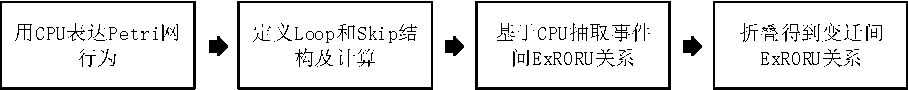
\includegraphics[width=1.0\textwidth]{exroru_procedure}
  \caption{ExRORU算法的基本流程\label{fig:exroru_procedure}}
\end{figure}

\textcolor{red}{
ExRORU计算步骤如下:
\begin{enumerate}[1.]
  \item 计算CPU。依据定义\ref{def:cpu},构造给定合理WF-net的CPU。
  \item 抽取事件间ExRORU关系。
\end{enumerate}
}

\section{ExRORU定义}\label{sec:exroru_definition}
本节主要介绍ExRORU的定义,首先介绍事件间的扩展不确定性精炼因果关系和并行关系,随后介绍变迁间的ExRORU关系。方便起见,约定$\Sigma=(P,T,F,M_{0})$是一个合理WF-net,$U=(B,E,A,f)$是其CPU。令$x,y\in E$是$U$的两个事件。示例WF-net及其CPU如图\ref{fig:case_study_petri}和图\ref{fig:case_study_cpu}所示。

\begin{figure}[htbp]
  \centering
  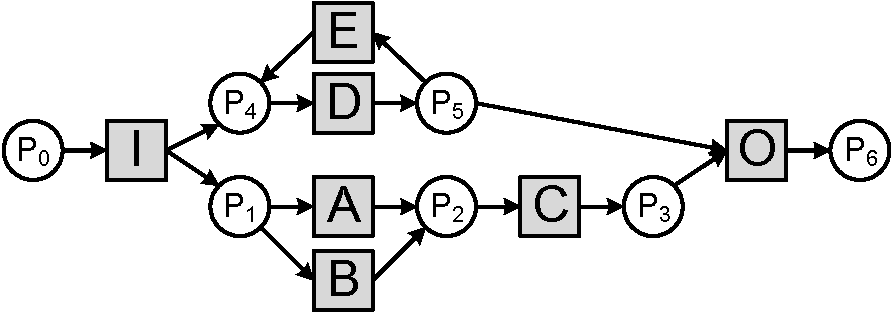
\includegraphics[width=0.7\textwidth]{case_study_petri}
  \caption{一个合理WF-net\label{fig:case_study_petri}}
\end{figure}

\begin{figure}[htbp]
  \centering
  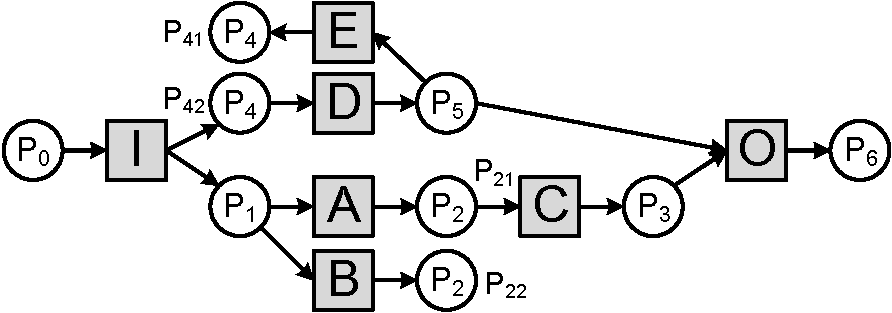
\includegraphics[width=0.7\textwidth]{case_study_cpu}
  \caption{图\ref{fig:case_study_petri}的CPU\label{fig:case_study_cpu}}
\end{figure}

\subsection{扩展不确定性精炼因果关系}
本文用形如$[ab\{c,d\}e]$的表达式来描述过程流的行为语义。连续出现的字母表示处于顺序结构中的事件;大括号中的表达式表示并行结构,其不同分支用逗号隔开。该表达式可以互相嵌套以表达复杂过程流的语义。例如在图\ref{fig:case_study_cpu}的CPU中,$[I\{D,AC\}O]$、$[I\{D,BC\}O]$和$[I\{DED,AC\}O]$是一些过程流表达式示例。

轨迹是一系列事件的有穷序列$\sigma\in E^{*}$,可以从网的初始状态开始按顺序执行其中的事件最终得到终止状态。令$\Omega$是$U$中所有过程流的轨迹集合。不可见事件/变迁是模型中起路由作用的无意义事件/变迁,在逻辑流中不被表达出来\cite{wen2007mining}。本文使用带斜线的阴影方框表示不可见事件/变迁,如图\ref{fig:sda_example}所示。基于两个事件是否能在一条轨迹中紧邻发生,首先定义直接和简介因果关系。

\begin{definition}[直接和间接因果关系]\label{def:d_i_causal_relation}
事件$x$和$y$满足因果关系,即$x<y$。它们满足直接因果关系当且仅当:$\exists\sigma=\langle e_{1},e_{2},...,e_{n}\rangle\in\Omega,1\leq i<j\leq n,e_{i}=x,e_{j}=y$,使得$\forall k\in(i,j)$,$e_{k}$是不可见事件。否则,$x$和$y$满足间接因果关系。
\end{definition}

\begin{example}
在图\ref{fig:case_study_cpu}的CPU中,事件$A$和$C$、事件$C$和$O$都满足直接因果关系而事件$A$和$O$满足间接因果关系。
\end{example}

令$\Uptheta$是经$U$展开得到的所有过程流集合,$\Uptheta_{x}$是$\Uptheta$中含有$x$的过程流子集,即$\Uptheta_{x}=\{\beta\in\Uptheta|x\in\beta\}$。$TS(\beta)$表示过程流$\beta$所有轨迹的集合。

\begin{definition}[扩展不确定性精炼因果关系]\label{def:exroru_causal}
事件$x$和$y$满足:
  \begin{itemize}
  	\item[-] 总是因果关系(always causal relation),记作$x\overset{\text{\tiny{A}}}{\rightarrow}y$,当且仅当:$x<y$且$\forall\beta_{x}\in\Uptheta_{x}$,$\forall\sigma\in TS(\beta_{x})$:在$x$被执行后,$y$必须被执行且在每两个$x$的执行之间(如果$\sigma$中有超过一个$x$)至少有一个$y$要被执行。
  	\item[-] 从不因果关系(never causal relation),记作$x\overset{\text{\tiny{N}}}{\rightarrow}y$,当且仅当:$\forall\beta_{x}\in\Uptheta_{x}$,$\forall\sigma\in TS(\beta_{x})$:当$x$被执行,$y$不能在其后被执行。
  	\item[-] 有时因果关系(sometimes causal relation),记作记作$x\overset{\text{\tiny{S}}}{\rightarrow}y$,当且仅当$x$和$y$不满足上述两种关系。
  \end{itemize}
\end{definition}

\section{本章小结}